\subsection{I3D (Inflated 3D ConvNets)}
\begin{frame}[allowframebreaks]{Inflating 2D Networks to 3D (I3D)}
    \begin{itemize}
        \item There has been a lot of work on architectures for images.
        \item Can we reuse image architectures for video?
        \item Idea: take a 2D CNN architecture.
        \item Replace each 2D $K_h \times K_w$ conv/pool layer with a 3D $K_t \times K_h \times K_w$ version.
        \item Can use weights of 2D conv to initialize 3D conv: copy $K_t$ times in space and divide by $K_t$.
        \item This gives the same result as 2D conv given ``constant'' video input.
    \end{itemize}
\framebreak
    \begin{itemize}
        \item \textbf{Introduced by Carreira and Zisserman, CVPR 2017} \\
        \item \textbf{Key Ideas:}
        \begin{itemize}
            \item \textbf{Inflation of 2D Filters}: Converts 2D convolutional filters into 3D by replicating them across time.
            \item \textbf{Temporal Modeling}: Captures motion information effectively by leveraging pre-trained 2D networks.
            \item \textbf{End-to-End Training}: Trained on large video datasets, allowing transfer learning to new tasks.
            \item \textbf{Performance Boost}: Significantly improves action recognition accuracy compared to previous methods.
        \end{itemize}
    \end{itemize}
\framebreak
    \begin{figure}
        \centering
        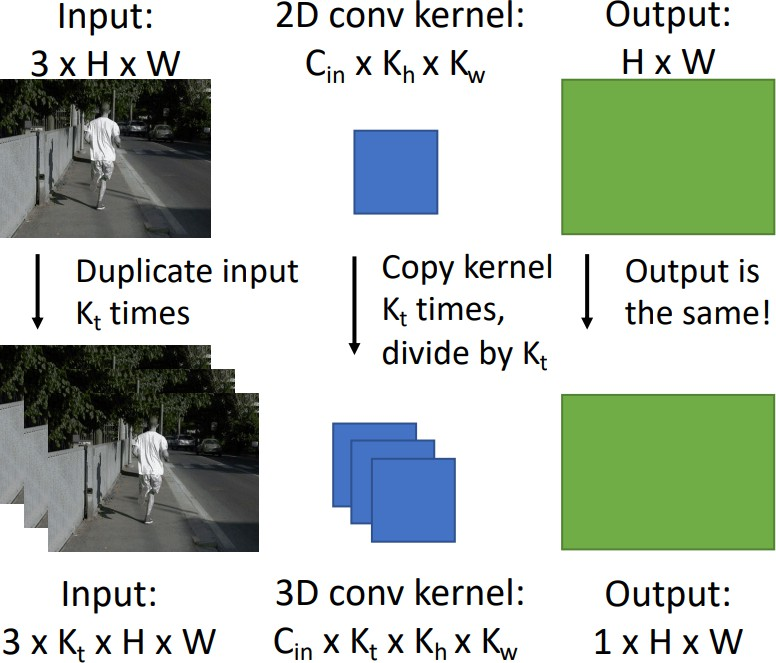
\includegraphics[width=1\textwidth,height=0.9\textheight,keepaspectratio]{images/video/slide_36_1_img.jpg}
    \end{figure}
\framebreak
    \begin{figure}
        \centering
        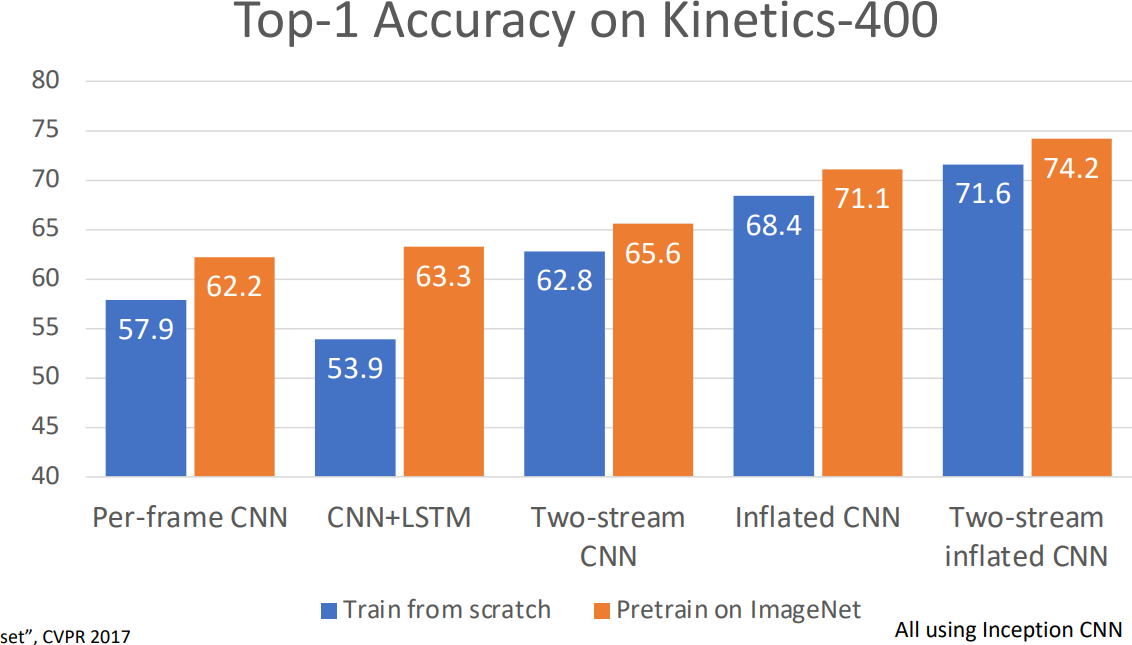
\includegraphics[width=1\textwidth,height=0.9\textheight,keepaspectratio]{images/video/slide_37_1_img.png}
    \end{figure}
\end{frame}